% =====================================================================
%  MEMoE: MoE-Oriented Memory Expansion
%  Team King Bob, Nebula 2026
%
%  Build:  pdflatex memoe.tex  (twice, for references)
%
%  Figures live in ../results/. The \graphicspath below picks them up.
%  Places marked SCREENSHOT need a capture pasted in; each one says
%  exactly what to capture.
% =====================================================================

\documentclass[11pt,a4paper]{article}

\usepackage[margin=2.4cm]{geometry}
\usepackage[T1]{fontenc}
\usepackage{lmodern}
\usepackage{microtype}
\usepackage{graphicx}
\usepackage{booktabs}
\usepackage{amsmath}
\usepackage{caption}
\usepackage{subcaption}
\usepackage{xcolor}
\usepackage{tikz}
\usetikzlibrary{arrows.meta,positioning,fit,backgrounds,calc,shapes.geometric}
\usepackage{titlesec}
\usepackage{enumitem}
\usepackage[colorlinks=true,linkcolor=linknavy,citecolor=linknavy,urlcolor=linknavy]{hyperref}

\definecolor{linknavy}{HTML}{1B4FA8}
\definecolor{rulegrey}{HTML}{DCE0E6}
\definecolor{inkmuted}{HTML}{5A6472}
\definecolor{boxfill}{HTML}{F4F6F8}

\captionsetup{font=small,labelfont=bf,labelsep=period}
\titleformat{\section}{\large\bfseries}{\thesection}{0.7em}{}
\titleformat{\subsection}{\normalsize\bfseries}{\thesubsection}{0.7em}{}
\setlist{itemsep=2pt,topsep=4pt}

\graphicspath{{../results/}{../results/figures/}{../results/figures_extra/}%
              {../results/figures_real/}{../results/figures_runtime/}{figures/}}

% =====================================================================
%  diagrams/tikzsetup.tex
%  Shared TikZ styles for the MEMoE diagrams. Input from memoe.tex after
%  the colour definitions (linknavy, rulegrey, inkmuted, boxfill) and
%  after \usetikzlibrary{...}.
% =====================================================================

\usetikzlibrary{patterns}

\definecolor{tierhot}{HTML}{C2703D}   % HBM / GPU-resident
\definecolor{tiercold}{HTML}{2E7D8A}  % host DRAM / CXL tier
\definecolor{stagefill}{HTML}{EEF3F6}
\definecolor{hotfill}{HTML}{FBEEE5}
\definecolor{coldfill}{HTML}{E7F1F3}

\tikzset{
  % ---- generic blocks -------------------------------------------------
  mnode/.style={
    draw=rulegrey, line width=0.6pt, fill=stagefill, rounded corners=2pt,
    minimum height=8mm, inner xsep=5pt, align=center,
    font=\footnotesize},
  mstage/.style={mnode, minimum width=26mm},
  mhot/.style={mnode, draw=tierhot, fill=hotfill},
  mcold/.style={mnode, draw=tiercold, fill=coldfill},
  mlabel/.style={font=\scriptsize\itshape, text=inkmuted, align=center},
  mtiny/.style={font=\scriptsize, text=inkmuted, align=center},
  % ---- connections ----------------------------------------------------
  mflow/.style={
    -{Stealth[length=4pt,width=3pt]}, draw=inkmuted, line width=0.6pt},
  mlink/.style={
    -{Stealth[length=4pt,width=3pt]}, draw=tiercold, line width=1.0pt},
  mdash/.style={mflow, dashed, dash pattern=on 2pt off 1.6pt},
  % ---- timeline bars --------------------------------------------------
  bar/.style={draw=rulegrey, line width=0.5pt, minimum height=5mm,
              inner sep=0pt, anchor=south west, font=\scriptsize},
  barcompute/.style={bar, fill=hotfill, draw=tierhot},
  barcopy/.style={bar, fill=coldfill, draw=tiercold},
  barstall/.style={bar, fill=white, draw=inkmuted,
                   pattern=north east lines},
  axis/.style={draw=inkmuted, line width=0.5pt},
}


% A box for the headline claims.
\newcommand{\keyresult}[1]{%
  \begin{center}\fcolorbox{rulegrey}{boxfill}{%
    \begin{minipage}{0.93\linewidth}\vspace{4pt}#1\vspace{4pt}\end{minipage}}%
  \end{center}}

% Placeholder marker for screenshots still to be pasted in.
\newcommand{\screenshot}[2]{%
  \begin{figure}[htbp]\centering
  \fcolorbox{rulegrey}{boxfill}{\begin{minipage}{0.92\linewidth}
  \vspace{2.2cm}\centering{\color{inkmuted}\small SCREENSHOT: #1}\vspace{2.2cm}
  \end{minipage}}
  \caption{#2}
  \end{figure}}

\title{\vspace{-1.4cm}\textbf{MEMoE: Memory Expansion for Mixture-of-Experts Inference}\\[4pt]
\large When a slow memory tier can hold the experts, and when it cannot}

\author{Team King Bob\\
\small Shashank Yammanuru \quad Shreyansh Jain \quad Kanav Sharma\\
\small BITS Pilani \quad$\cdot$\quad Nebula 2026, Software Category}

\date{\small September 2026}

\begin{document}
\maketitle

\begin{abstract}
\noindent
Mixture-of-Experts models decouple capacity from compute: DeepSeek-V3 holds 671
billion parameters but activates roughly 37 billion per token. The unused
parameters still have to live in GPU memory, so the model needs sixteen H100s to
hold weights that only require the arithmetic of about two. We ask whether a
slower, larger memory tier can hold the idle experts instead, and at what cost.

We answer with measurements rather than models alone. We characterised a CXL-class
tier in DRAMSim3, captured 258{,}629 tokens of real routing from OLMoE-1B-7B across
four workloads, and built MEMoE-RT, a runtime that executes the checkpoint with
its expert weights held outside GPU memory and streamed in over PCIe while
attention computes.

Three measurements redirected the design. Expert coverage saturates by a batch of
about one thousand tokens, so the fast tier stops behaving as a cache. Fetch hit
rate then equals the resident fraction exactly, at every routing skew we tested,
which makes popularity-based placement worthless. And hot expert sets are
anti-correlated across domains, so a placement profiled on prose serves code worse
than random placement does. Together these rule out the tiering engine the
literature reaches for, and leave a capacity decision plus a bandwidth window
scheduling problem.

MEMoE-RT confirms the resulting design on hardware. At a prefill batch of 16{,}384
tokens it runs with all 64 experts per layer held off-GPU, using 7.27~GB instead of
17.73~GB of GPU memory, and retains 91.9\% of fully resident throughput. At a
decode-sized batch of 512 tokens the same configuration retains 38.3\%. Our closed
form for the critical batch size, derived before any of these runs, predicts the
observed crossover to within 0.5\%.
\end{abstract}

\vspace{4pt}
\hrule
\vspace{10pt}

% =====================================================================
\section{The problem}
% =====================================================================

A Mixture-of-Experts layer replaces one feed-forward network with many. A router
picks a few per token, so compute stays roughly constant while parameter count
grows. The economics are attractive until deployment, because every expert must
be addressable by the GPU even though almost none are used at any instant.

Table~\ref{tab:footprint} makes the imbalance concrete. Across the four
checkpoints we studied, routed experts account for between 93.1\% and 97.5\% of
all parameters. DeepSeek-V3 needs sixteen 80~GB devices to hold 1{,}249~GB of
weights, of which 1{,}218~GB are experts sitting idle. The GPUs are bought for
capacity, not for arithmetic.

\begin{table}[htbp]
\centering\small
\caption{Weights and expert pool in GB, from our footprint model, validated
against published parameter counts. GPU counts assume 80~GB of HBM per device,
and 512~GB of a secondary tier per device in the last column.}
\label{tab:footprint}
\begin{tabular}{lrrrrr}
\toprule
Model & Weights & Expert pool & Experts & GPUs, HBM & GPUs, tiered \\
\midrule
OLMoE-1B-7B     & 12.9   & 12.0   & 93.1\% & 1  & 1 \\
Mixtral-8x7B    & 87.0   & 84.0   & 96.6\% & 2  & 1 \\
Qwen3-235B-A22B & 437.8  & 423.0  & 96.6\% & 6  & 1 \\
DeepSeek-V3     & 1249.2 & 1218.0 & 97.5\% & 16 & 3 \\
\bottomrule
\end{tabular}
\end{table}

Compute Express Link offers a way out. A CXL Type-3 expander attaches DRAM over a
link, giving hundreds of gigabytes per node at a fraction of the cost of HBM, and
at a fraction of the bandwidth. The obvious plan is to keep popular experts in
fast memory and fetch the rest on demand. We set out to build that, and the
measurements sent us somewhere else.

This report describes what we measured, why it changed the design, and what the
resulting system does on real hardware.

% =====================================================================
\section{What we built}
% =====================================================================

MEMoE is a measurement stack and a runtime.

\begin{itemize}
\item \textbf{A footprint model} that reads checkpoint configurations and reports
      expert pool size, KV cache growth, and device counts under a given memory
      budget.
\item \textbf{A tier characterisation} in DRAMSim3, which measures what a CXL-class
      DRAM back end actually sustains for bulk expert reads rather than quoting a
      DIMM rating.
\item \textbf{A routing capture} that hooks the router of a live checkpoint and
      records which experts fire for every token, across four workloads.
\item \textbf{A trace-driven simulator} that replays those traces against placement
      policies, residency levels, and prefetch depths.
\item \textbf{Closed-form analyses} for the critical batch size, the expert versus
      KV cache question, pooling, and transfer granularity.
\item \textbf{MEMoE-RT}, a runtime that executes OLMoE-1B-7B with its expert
      weights outside GPU memory, streaming them over PCIe on a dedicated copy
      stream while attention computes on the main one.
\item \textbf{A CXL software path investigation} in QEMU, which reached full device
      enumeration and decoder programming before hitting a kernel gate that cannot
      be passed inside a virtual machine.
\item \textbf{An interactive dashboard} that presents every result above and lets a
      reader put their own model and hardware into the capacity formula.
\end{itemize}

The runtime is what turns the rest from a spreadsheet into an instrument. Because
we can measure end-to-end throughput on hardware, we can check whether the
analytical model predicts reality, and it does.

% =====================================================================
%  diagrams/method.tex  --  how the pieces feed each other
% =====================================================================
\begin{figure}[htbp]
\centering
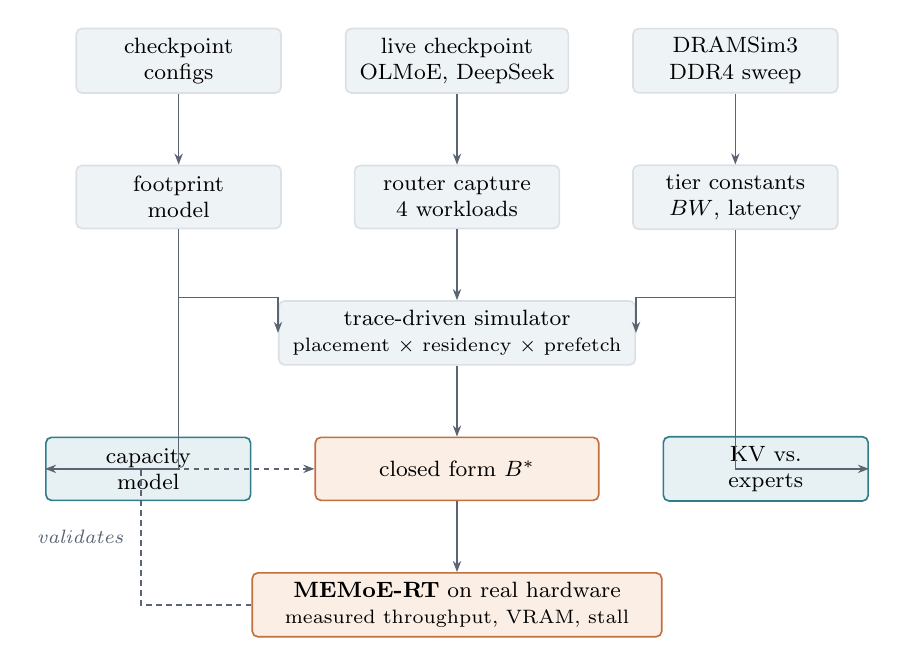
\begin{tikzpicture}[node distance=4mm]

% ---- row 1: inputs ---------------------------------------------------
\node[mstage] (cfg)  {checkpoint\\configs};
\node[mstage, right=8mm of cfg] (ckpt) {live checkpoint\\OLMoE, DeepSeek};
\node[mstage, right=8mm of ckpt] (dram) {DRAMSim3\\DDR4 sweep};

% ---- row 2: derived --------------------------------------------------
\node[mstage, below=9mm of cfg]  (foot) {footprint\\model};
\node[mstage, below=9mm of ckpt] (hook) {router capture\\4 workloads};
\node[mstage, below=9mm of dram] (tier) {tier constants\\$BW$, latency};

% ---- row 3: the simulator -------------------------------------------
\node[mstage, below=9mm of hook, minimum width=44mm] (sim)
  {trace-driven simulator\\\scriptsize placement $\times$ residency $\times$ prefetch};

% ---- row 4: outputs --------------------------------------------------
\node[mhot, below=9mm of sim, minimum width=36mm] (closed)
  {closed form $B^{*}$};
\node[mcold, left=8mm of closed, minimum width=26mm] (cap)
  {capacity\\model};
\node[mcold, right=8mm of closed, minimum width=26mm] (kv)
  {KV vs.\\experts};

% ---- row 5: the runtime ---------------------------------------------
\node[mhot, below=9mm of closed, minimum width=52mm] (rt)
  {\textbf{MEMoE-RT} on real hardware\\\scriptsize measured throughput, VRAM, stall};

% ---- edges -----------------------------------------------------------
\draw[mflow] (cfg)  -- (foot);
\draw[mflow] (ckpt) -- (hook);
\draw[mflow] (dram) -- (tier);

\draw[mflow] (hook) -- (sim);
\draw[mflow] (foot.south) |- ([yshift=4.5mm]sim.west) -- (sim.west);
\draw[mflow] (tier.south) |- ([yshift=4.5mm]sim.east) -- (sim.east);

\draw[mflow] (sim) -- (closed);
\draw[mflow] (foot.south) |- (cap.west);
\draw[mflow] (tier.south) |- (kv.east);

\draw[mflow] (closed) -- (rt);
\draw[mdash] (rt.west) -- ++(-14mm,0) |- (closed.west)
  node[mlabel, pos=0.25, left=1mm] {validates};

\end{tikzpicture}
\caption{How the components feed each other. Everything above the runtime is
analysis or simulation; the runtime is the only part that touches real weights on
a real device, and it is what checks the closed form against measured behaviour.}
\label{fig:method}
\end{figure}


\screenshot{The MEMoE dashboard, summary section, showing the three measured
constants and the three findings}{The dashboard presents every result in this
report and includes a live calculator for the critical batch size.
Available at \texttt{results/dashboard.html}.}

% =====================================================================
\section{Characterising the tier}
% =====================================================================

We did not want to quote CXL bandwidth from a datasheet. A Type-3 expander is DRAM
behind a controller, so we simulated the DRAM directly and read the rate it
sustained while busy. Traces were 12~MB sequential reads, the size of one OLMoE
expert, issued as 196{,}608 accesses of 64 bytes.

\begin{table}[htbp]
\centering\small
\caption{DRAMSim3, DDR4 x8, 12~MB sequential expert read. Sustained bandwidth is
computed from average interarrival time, not from the headline figure, which is
diluted by idle cycles between requests.}
\label{tab:dram}
\begin{tabular}{lrrrr}
\toprule
Grade & Specification & Sustained & Share reached & Loaded latency \\
\midrule
DDR4-1866 & 14.9 GB/s & 12.76 GB/s & 85.5\% & 237.9 ns \\
DDR4-2133 & 17.1 GB/s & 13.24 GB/s & 77.6\% & 228.9 ns \\
DDR4-2400 & 19.2 GB/s & 14.96 GB/s & 77.9\% & 202.9 ns \\
DDR4-2666 & 21.3 GB/s & 15.29 GB/s & 71.7\% & 197.3 ns \\
DDR4-2933 & 23.5 GB/s & 15.65 GB/s & 66.7\% & 192.9 ns \\
DDR4-3200 & 25.6 GB/s & \textbf{16.88 GB/s} & 65.9\% & \textbf{179.4 ns} \\
\bottomrule
\end{tabular}
\end{table}

Two things are worth taking from Table~\ref{tab:dram}. The first is the headline
figure of 16.88~GB/s, which we use everywhere in place of a specification number.
The second is the trend: efficiency falls from 85.5\% to 65.9\% as the grade
rises, because timing constraints such as tRC, tFAW and refresh do not scale with
the data rate. Anyone specifying an expander should budget against sustained
bandwidth, not DIMM peak, and the gap widens with faster parts.

One number in this section is derived rather than directly measured.
Multi-channel configurations did not scale in DRAMSim3 even with address mapping
interleaving correctly, because its trace driver issues at most one request per
cycle and starves the extra channels. Where a four-channel figure appears in this
report it is the measured single channel multiplied by four. Section~9.2 tests
that multiplication in gem5, which has no such issue-rate limit, and finds
scaling linear to four channels within 0.03\%.

\begin{figure}[htbp]
\centering
\includegraphics[width=0.86\linewidth]{f1_bandwidth.png}
\caption{Sustained bandwidth against DIMM specification across DDR4 grades. The
gap is the part a capacity plan has to account for.}
\label{fig:dram}
\end{figure}

% =====================================================================
\section{How real routing behaves}
% =====================================================================

Every argument about expert tiering rests on an assumption about routing skew, so
we measured it instead of assuming it. We registered forward hooks on the router
of OLMoE-1B-7B-0924-Instruct and recorded the selected experts for every token
across four workloads: prose, mathematics, code, and chat. The capture totals
258{,}629 tokens.

\subsection{Skew is a property of the input}

\begin{table}[htbp]
\centering\small
\caption{Routing statistics per workload, same model and same weights throughout.
Normalised entropy of 1.0 would be perfectly uniform.}
\label{tab:skew}
\begin{tabular}{lrrrrr}
\toprule
Workload & Tokens & Zipf $s$ & Entropy & Gini & Top quarter \\
\midrule
chat  & 18{,}239  & 0.494 & 0.972 & 0.261 & 40.7\% \\
prose & 37{,}355  & 0.598 & 0.963 & 0.300 & 43.5\% \\
math  & 63{,}257  & 0.899 & 0.913 & 0.442 & 56.0\% \\
code  & 139{,}778 & 1.132 & 0.877 & 0.522 & 63.6\% \\
\bottomrule
\end{tabular}
\end{table}

Skew varies by a factor of 2.3 between chat and code on identical weights. Chat
routing is close to uniform, with no expert taking more than 4\% of routings,
which is what a load-balancing auxiliary loss during training is designed to
produce. Any system that assumes a fixed skew will be tuned for one workload and
wrong for another.

\subsection{Coverage saturates before serving begins}

The case for expert tiering depends on reuse: if a batch touches only some
experts, the rest need not be resident. We measured how many experts a batch
touches per layer as batch size grows.

\begin{figure}[htbp]
\centering
\includegraphics[width=0.86\linewidth]{f3_coverage.png}
\caption{Share of experts touched per layer against batch size, from the captured
traces. By 1{,}024 tokens every workload is at or near total coverage.}
\label{fig:coverage}
\end{figure}

By a batch of 1{,}024 tokens, coverage reaches 97.3\% to 100\% depending on the
workload. Past that point every non-resident expert is fetched on every batch,
forever. There is no reuse distance left to shorten and the fast tier stops
behaving as a cache: it is a fixed partition.

Both real serving regimes sit inside the saturated zone. Continuous batching
during decode runs 64 to 256 concurrent sequences. Prefill runs thousands of
tokens at once. Neither is small batch.

\subsection{Popularity buys nothing}

If every expert is touched, ranking them by popularity should not help. We tested
this by sweeping synthetic routing from perfectly uniform to more skewed than
anything we measured, at 90\% residency.

\begin{table}[htbp]
\centering\small
\caption{Fetch hit rate at 90\% residency across routing skew. At batch 512 and
above the hit rate equals the resident fraction exactly.}
\label{tab:skewsweep}
\begin{tabular}{lrrrr}
\toprule
Batch & $s=0.0$ & $s=0.6$ & $s=1.0$ & $s=1.5$ \\
\midrule
64    & 0.899 & 0.900 & 0.907 & 0.927 \\
512   & 0.899 & 0.899 & 0.899 & 0.899 \\
8192  & 0.899 & 0.899 & 0.899 & 0.899 \\
\bottomrule
\end{tabular}
\end{table}

Static placement, LRU and sampled LFU all perform identically at serving batch
sizes. This is convenient rather than disappointing: static placement is decided
once at load time and costs nothing on the critical path, so the cheapest policy
is also the best available one.

\subsection{The wrong profile is worse than none}

If placement cannot help, can it hurt? We took the top quarter of experts for each
workload and measured overlap between workloads, using a split-half control on the
same workload to establish that the measurement is meaningful at all.

\begin{figure}[htbp]
\centering
\begin{subfigure}{0.48\linewidth}
  \includegraphics[width=\linewidth]{e2_overlap.png}
  \caption{Hot set overlap. Chance is 25\%.}
\end{subfigure}\hfill
\begin{subfigure}{0.48\linewidth}
  \includegraphics[width=\linewidth]{e3_penalty.png}
  \caption{Cross-workload hit rate at 50\% residency. Random scores 0.500.}
\end{subfigure}
\caption{Hot expert sets split into two camps. Prose and chat share experts;
mathematics and code share experts; across the two groups overlap falls below
chance.}
\label{fig:overlap}
\end{figure}

Self-overlap runs from 75.0\% to 94.9\%, so the hot sets are stable within a
workload. Across workloads, mathematics and code overlap 50.0\%, while prose and
code overlap 15.2\%, well below the 25\% expected by chance. Code routes to
experts that prose actively avoids.

The consequence is measured in the right-hand panel. A placement profiled on prose
and then asked to serve code achieves a hit rate of 0.383, against 0.500 for
random placement. Profiling on the wrong workload is worse than not profiling.

This is domain specialisation visible in routing statistics alone, from 260{,}000
tokens on a 7B model, with no interpretability tooling. For mixed serving traffic
it means there is no good static expert placement, and the resident set should be
chosen by capacity alone.

% =====================================================================
\section{The capacity model}
% =====================================================================

Since skew is irrelevant and policy choice is irrelevant, two decisions remain:
how much fast memory to buy, and how early to start the transfer. The first has a
closed form.

Let $E$ be experts per layer, $k$ experts activated per token, $h$ the share of
fetches the resident tier covers, $F$ per-GPU compute in FLOP/s, $BW$ tier
bandwidth in bytes per second, and $\varepsilon$ the throughput loss to be
tolerated. Fetch traffic per layer is proportional to $(1-h)E$ times expert size,
while compute per layer is proportional to $Bk$ times expert size. Expert size
cancels, giving the batch size at which transfer time falls within the stall
budget:

\begin{equation}
B^{*} = \frac{(1-h)\,E\,F}{BW \cdot k \cdot \varepsilon}
\label{eq:bstar}
\end{equation}

Two properties make Equation~\ref{eq:bstar} useful. It does not depend on expert
size, because a larger expert costs proportionally more to move and does
proportionally more work once moved. And it does not depend on GPU count, because
compute and per-node bandwidth scale together under tensor parallelism. Scaling
out does not get you past it.

\keyresult{\textbf{The prediction.} Calibrating $F$ from the fully resident
baseline alone gives 33.7~TFLOPS for our GPU on this workload. Substituting
$h=0.3$, $E=64$, $k=8$, $BW=40.8$~GB/s and $\varepsilon=1$ into
Equation~\ref{eq:bstar} predicts a crossover at $B^{*}=4{,}626$ tokens. The
offload runs, which played no part in the calibration, place the observed
crossover at 4{,}645 tokens. The agreement is 0.5\%.}

% =====================================================================
\section{Experts, not the KV cache}
% =====================================================================

The KV cache is the other structure that destroys HBM budgets, so we asked whether
it is also a candidate for the slow tier. It is not, and the reason generalises.

A tier with bandwidth $BW$ feeding a device at $F$ FLOP/s is balanced at $F/BW$
FLOPs per byte; below that ratio the workload is bandwidth bound. Each fetched
expert serves $Bk/E$ tokens, so expert arithmetic intensity \emph{grows with the
batch}. Each cached KV element is read once per decode step and consumed by
$n_{\text{heads}}/n_{\text{kv heads}}$ query heads, so KV intensity is
\emph{fixed}. Batching cannot rescue it, because every sequence brings its own KV.

\begin{table}[htbp]
\centering\small
\caption{Arithmetic intensity in FLOPs per byte. The balance point for a
four-channel tier is 5{,}861. Qwen3 has the best KV intensity in the set through
16-to-1 grouped query attention, and is still 366 times below it.}
\label{tab:kv}
\begin{tabular}{lrrr}
\toprule
Model & KV intensity & Balance point & Batch for expert parity \\
\midrule
OLMoE-1B-7B     & 1.0  & 5{,}861 & 46{,}886 \\
Mixtral-8x7B    & 4.0  & 5{,}861 & 23{,}443 \\
Qwen3-235B-A22B & 16.0 & 5{,}861 & 93{,}772 \\
DeepSeek-V3     & 1.0  & 5{,}861 & 166{,}706 \\
\bottomrule
\end{tabular}
\end{table}

Concretely, one 32k-context Qwen3 sequence reads 5.875~GB of KV per decode step.
On HBM3e that is 1.883~ms, or 531 steps per second. On a four-channel CXL tier it
is 93.455~ms, or 11 steps per second: a 48-fold slowdown. Active KV must stay in
HBM.

Cold KV is a separate question. Preempted requests and prefix caches are not read
every step and may tier well, but we did not model that and do not claim it.

% =====================================================================
\section{MEMoE-RT: the system}
% =====================================================================

The results above are all simulation or analysis. To test them we built a runtime
that runs the real checkpoint with its experts elsewhere.

\subsection{Design}

The design follows from the findings rather than from the literature.

Because coverage saturates, every expert in a layer will be needed. Prediction is
therefore trivial and the entire problem is scheduling the transfer early enough.
MEMoE-RT does not fetch experts individually on demand. It moves every
non-resident expert of layer $L+d$ as one contiguous transfer, issued $d$ layers
ahead, on a dedicated copy stream that overlaps with attention compute on the main
stream.

Because popularity is irrelevant, the resident set is simply the low expert
indices. There is deliberately no ranking anywhere in the implementation.

Because latency is negligible at expert granularity and dominant below it, we move
whole layers rather than fragments. We confirmed this on the target hardware
before building: 4~MB transfers reach 33.05~GB/s, 12~MB reach 36.67~GB/s, and the
plateau is 40.81~GB/s. A whole-layer transfer of roughly 480~MB sits on the
plateau.

Offloaded experts live in pinned host memory, laid out so that one layer's experts
are contiguous. A ring of $d+1$ GPU staging buffers receives them. Layer $L$ uses
slot $L \bmod (d+1)$, and the prefetch issued at layer $L$ targets $L+d$, whose
slot belongs to layer $L-1$ and has already been consumed. All waiting is done
GPU-side with stream events rather than host synchronisation, so the copy genuinely
overlaps compute, and stall time is measured by recording CUDA events either side
of the wait.

% =====================================================================
%  diagrams/arch.tex  --  MEMoE-RT data path
% =====================================================================
\begin{figure}[htbp]
\centering
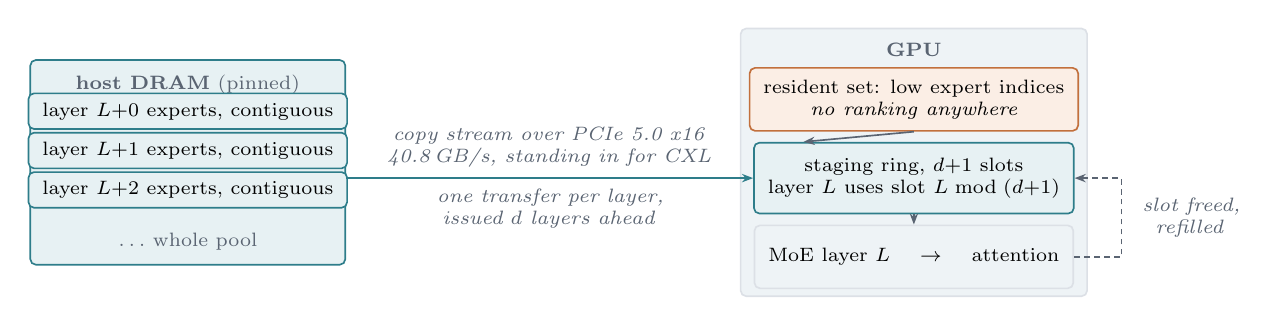
\begin{tikzpicture}

% ---------------- host side ------------------------------------------
\node[mcold, minimum width=40mm, minimum height=26mm, align=center] (host)
  {\ };
\node[mtiny, anchor=north] at ([yshift=-2pt]host.north)
  {\textbf{host DRAM} (pinned)};

\foreach \i/\y in {0/6.5mm, 1/1.5mm, 2/-3.5mm}{
  \node[mcold, minimum width=32mm, minimum height=4mm, font=\scriptsize]
       at ([yshift=\y]host.center) {layer $L{+}\i$ experts, contiguous};
}
\node[mtiny, anchor=south] at ([yshift=2pt]host.south) {$\ldots$ whole pool};

% ---------------- device side ----------------------------------------
\node[mnode, minimum width=44mm, minimum height=34mm, right=50mm of host] (gpu)
  {\ };
\node[mtiny, anchor=north] at ([yshift=-2pt]gpu.north) {\textbf{GPU}};

\node[mhot, minimum width=36mm, font=\scriptsize] (resident)
  at ([yshift=8mm]gpu.center)
  {resident set: low expert indices\\\itshape no ranking anywhere};

\node[mcold, minimum width=36mm, minimum height=9mm, font=\scriptsize] (ring)
  at ([yshift=-2mm]gpu.center)
  {staging ring, $d{+}1$ slots\\layer $L$ uses slot $L \bmod (d{+}1)$};

\node[mnode, minimum width=36mm, font=\scriptsize] (compute)
  at ([yshift=-12mm]gpu.center)
  {MoE layer $L$ \quad $\to$ \quad attention};

% ---------------- streams --------------------------------------------
\draw[mlink] (host.east |- ring.west) -- node[mlabel, above, pos=0.5, text width=44mm]
  {copy stream over PCIe 5.0 x16\\40.8\,GB/s, standing in for CXL}
  node[mlabel, below, pos=0.5, text width=44mm]
  {one transfer per layer,\\issued $d$ layers ahead} (ring.west);

\draw[mflow] (ring.south) -- (compute.north);
\draw[mflow] (resident.south) -- ([xshift=-14mm]ring.north);

\draw[mdash] (compute.east) -- ++(6mm,0) |- (ring.east)
  node[mlabel, pos=0.25, right=1mm, text width=13mm]
  {slot freed, refilled};

\end{tikzpicture}
\caption{MEMoE-RT data path. Non-resident experts live contiguously in pinned host
memory and move one whole layer at a time over a dedicated copy stream into a ring
of staging buffers, $d$ layers ahead of use. Waiting is done GPU-side with stream
events, so the transfer overlaps attention compute rather than serialising with
it.}
\label{fig:arch}
\end{figure}

% =====================================================================
%  diagrams/timeline.tex  --  two-stream overlap, d = 2
% =====================================================================
\begin{figure}[htbp]
\centering
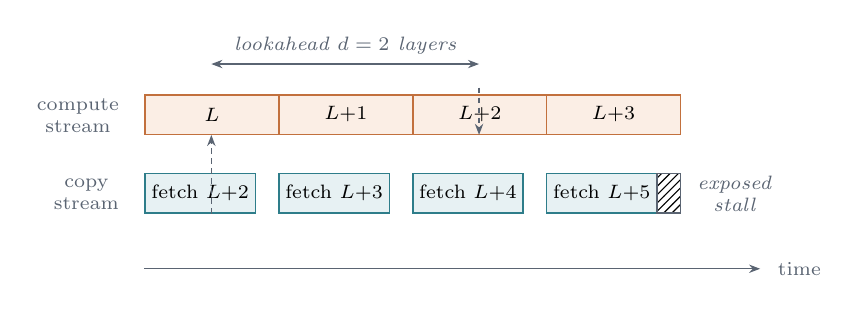
\begin{tikzpicture}[x=1mm, y=1mm]

\def\unit{17}      % width of one layer slot
\def\rowc{14}      % compute row y
\def\rowk{4}       % copy row y

% ---- row labels ------------------------------------------------------
\node[mtiny, anchor=east] at (-2, \rowc+2.5) {compute\\stream};
\node[mtiny, anchor=east] at (-2, \rowk+2.5) {copy\\stream};

% ---- compute row -----------------------------------------------------
\foreach \i/\lab in {0/$L$, 1/$L{+}1$, 2/$L{+}2$, 3/$L{+}3$}{
  \node[barcompute, minimum width=\unit mm] at (\i*\unit, \rowc) {\lab};
}

% ---- copy row: transfer for L+2 issued while L computes --------------
\foreach \i/\lab in {0/{fetch $L{+}2$}, 1/{fetch $L{+}3$},
                     2/{fetch $L{+}4$}, 3/{fetch $L{+}5$}}{
  \node[barcopy, minimum width=\unit mm - 3mm] at (\i*\unit, \rowk) {\scriptsize\lab};
}

% ---- exposed stall on the last one -----------------------------------
\node[barstall, minimum width=3mm] at (3*\unit + \unit - 3, \rowk) {};
\node[mlabel, anchor=west] at (4*\unit + 1, \rowk+2.5) {exposed\\stall};

% ---- lookahead annotation -------------------------------------------
\draw[mdash] (0.5*\unit, \rowk) -- (0.5*\unit, \rowc);
\draw[{Stealth[length=4pt]}-{Stealth[length=4pt]}, draw=inkmuted, line width=0.5pt]
  (0.5*\unit, \rowc+9) -- (2.5*\unit, \rowc+9)
  node[mlabel, midway, above] {lookahead $d = 2$ layers};
\draw[mdash] (2.5*\unit, \rowc+6) -- (2.5*\unit, \rowc);

% ---- time axis -------------------------------------------------------
\draw[axis, -{Stealth[length=4pt]}] (0, -3) -- (4.6*\unit, -3)
  node[mtiny, anchor=west, xshift=1mm] {time};

\end{tikzpicture}
\caption{Two-stream execution with lookahead $d=2$. The transfer for layer $L{+}2$
is issued while layer $L$ computes, so a fetch has two layers of compute to hide
behind. Roughly 60\% of transfer time hides in practice; the hatched remainder is
what the measured stall fraction reports.}
\label{fig:timeline}
\end{figure}


\subsection{Substituting PCIe for CXL}

We do not have CXL silicon, and neither does anyone outside a small number of
vendor labs. Host DRAM over PCIe is the standard substitute and is what we use: a
large, slow, byte-addressable tier behind a link. At PCIe 5.0 x16 the measured
plateau of 40.8~GB/s falls between our measured single-channel CXL figure of
16.88~GB/s and our scaled four-channel figure of 67.5~GB/s.

It is not CXL. It has different latency characteristics and no cache coherence.
What it reproduces faithfully is the structure of the problem, which is what the
analytical model is about.

\subsection{Correctness}

Every result below was checked against the reference implementation on identical
inputs. Tiered output agrees with the unmodified model to within one unit in the
last place of bfloat16 at the first layer, growing to 1.84 at the final layer
through sixteen layers of accumulation, with 92.8\% argmax agreement on random
token sequences. Per-layer divergence traces cleanly to rounding: CUDA
\texttt{index\_add\_} accumulates in nondeterministic order, and in bfloat16 that
changes the last bit. Two identical reference passes agree exactly, so the
comparison is meaningful.

\screenshot{Terminal output of \texttt{bench\_runtime.py --check} showing PASS}
{Correctness check comparing tiered execution against the reference
implementation before any timing result is taken.}

% =====================================================================
\section{What the runtime measures}
% =====================================================================

All runs use OLMoE-1B-7B in bfloat16 on an RTX PRO 4500 Blackwell with 32.6~GB of
memory over PCIe 5.0 x16, three repetitions per configuration, sequence length
512.

\subsection{The cost of offloading}

\begin{table}[htbp]
\centering\small
\caption{Residency sweep at batch 4{,}096. Throughput is relative to the fully
resident baseline of 20{,}917 tokens per second.}
\label{tab:residency}
\begin{tabular}{rrrrrr}
\toprule
Residency & Experts off-GPU & GPU memory & Tokens/s & Retained & Stalled \\
\midrule
1.00 & 0\%     & 14.84 GB & 20{,}917 & 100.0\% & 0.0\% \\
0.60 & 40.6\%  & 10.59 GB & 16{,}972 & 81.1\%  &  --   \\
0.40 & 59.4\%  &  8.62 GB & 15{,}062 & 72.0\%  &  --   \\
0.30 & 70.3\%  &  7.48 GB & 15{,}342 & 73.3\%  & 3.2\% \\
0.20 & 79.7\%  &  6.50 GB & 14{,}170 & 67.7\%  & 6.8\% \\
0.10 & 90.6\%  &  5.35 GB & 12{,}745 & 60.9\%  & 15.2\% \\
0.00 & 100\%   &  4.37 GB & 11{,}538 & 55.2\%  & 21.2\% \\
\bottomrule
\end{tabular}
\end{table}

\begin{figure}[htbp]
\centering

\includegraphics[width=0.88\linewidth]{r1_residency.png}
\caption{Throughput and GPU memory against the share of experts held off-GPU, at
batch 4{,}096. Memory falls faster than throughput across the whole range.}
\label{fig:residency}
\end{figure}

Run-to-run variation across repeated configurations is approximately
$\pm 3\%$, which is why the 0.30 row appears marginally above 0.40.

\subsection{The regime boundary}

The batch sweep is the central result, because it measures directly what the rest
of the report argues.

\begin{table}[htbp]
\centering\small
\caption{Batch sweep with 70\% of experts held off-GPU in every row. Baselines are
matched at each batch size.}
\label{tab:batch}
\begin{tabular}{rrrrr}
\toprule
Batch & Baseline tok/s & Tiered tok/s & Retained & Stalled \\
\midrule
512     &  5{,}340 &  2{,}046 & 38.3\% & 31.6\% \\
1{,}024 &  9{,}194 &  3{,}771 & 41.0\% & 26.5\% \\
4{,}096 & 20{,}917 & 14{,}614 & 69.9\% &  2.6\% \\
16{,}384 & 26{,}873 & 25{,}367 & \textbf{94.4\%} & 0.07\% \\
\bottomrule
\end{tabular}
\end{table}

\begin{figure}[htbp]
\centering

\includegraphics[width=0.88\linewidth]{r2_batch_regime.png}
\caption{Retention and stall against batch size with a fixed 70\% of experts
off-GPU. The transition sits between the decode and prefill regimes, where
Equation~\ref{eq:bstar} predicts it.}
\label{fig:batch}
\end{figure}

The same configuration costs 62\% of throughput at a decode-sized batch and 5.6\%
at a prefill-sized one. This is the claim that expert offload is a prefill
technique, stated as a measurement rather than an argument.

Pushing further, at batch 16{,}384 with \emph{all} experts off-GPU:

\keyresult{\textbf{The headline.} With all 64 experts per layer held outside GPU
memory, that is 93\% of the model's parameters, MEMoE-RT sustains 24{,}684 tokens
per second against a fully resident baseline of 26{,}873, or \textbf{91.9\%}. GPU
memory falls from 17.73~GB to 7.27~GB, a \textbf{2.44-fold reduction}. Time
stalled on transfer is 0.67\%.}

\subsection{Lookahead depth, and a correction}

Our simulation work recommended a prefetch depth of 4 to 8 layers. The hardware
disagrees.

\begin{table}[htbp]
\centering\small
\caption{Depth sweep at 59.4\% offload, batch 4{,}096. Throughput is flat while
staging memory grows 41\%.}
\label{tab:depth}
\begin{tabular}{rrrr}
\toprule
Lookahead & Tokens/s & GPU memory & Stalled \\
\midrule
1 & 14{,}798 &  8.14 GB & 2.4\% \\
2 & 14{,}926 &  8.62 GB & 2.3\% \\
4 & 14{,}681 &  9.58 GB & 2.3\% \\
8 & 14{,}238 & 11.49 GB & 2.3\% \\
\bottomrule
\end{tabular}
\end{table}

\begin{figure}[htbp]
\centering

\includegraphics[width=0.85\linewidth]{r3_depth.png}
\caption{Deeper lookahead buys no throughput once transfers are batched per layer,
and costs staging memory.}
\label{fig:depth}
\end{figure}

The explanation is our own design change. The simulator modelled per-expert
on-demand fetches, which need deep lookahead to stay ahead of demand. The runtime
moves a whole layer in one transfer, and at this operating point layer transfer
time and layer compute time are close to equal, so a single layer of lookahead
already covers the gap. Batching the transfer removed the need for depth.

We report the correction rather than the original recommendation. Depth 1 is
sufficient, and depth 8 wastes 41\% more staging memory for slightly less
throughput.

\subsection{Calibrating the overlap assumption}

The analytical model assumes transfer hides perfectly under compute. Fitting
measured wall time to $t = t_{\text{compute}} + \kappa \cdot t_{\text{transfer}}$
across the residency sweep gives $\kappa = 0.40 \pm 0.07$.

\begin{figure}[htbp]
\centering

\includegraphics[width=0.88\linewidth]{r4_overlap.png}
\caption{Measured wall time against the perfect-overlap model and the fitted one.
Roughly 60\% of transfer time hides under compute; the remaining 40\% is exposed.}
\label{fig:overlap}
\end{figure}

So about 60\% of transfer time is hidden and 40\% is not. The ideal model
over-predicts throughput by up to 40\% where transfer and compute are balanced.
This is copy engine and compute contention, which our earlier work listed as its
clearest unmodelled gap. It is now a measured constant, and multiplying predicted
transfer exposure by $\kappa$ brings the analytical model into agreement with
hardware across the full sweep.

% =====================================================================
\section{Two smaller results}
% =====================================================================

\subsection{Pooling trades capacity for batch size, one for one}

If $N$ nodes share one copy of the cold experts, they save $N$ times the capacity
but contend for one link, so per-node bandwidth falls as $1/N$. Since $B^{*}$ is
inversely proportional to bandwidth, both move together at exactly the same rate.

For Qwen3-235B against a 67.5~GB/s pool, sixteen nodes save 6.3~TB and require a
1.5 million token batch, which is not a real operating point. Pooling is worth it
at small $N$, or when the pool link scales with membership. The latter is what CXL
3.0 switching promises, and it is precisely the part that is pre-production, so we
model it and label it as modelled.

\subsection{Fetch whole experts}

At 300~ns access latency, the share of transfer time spent waiting rather than
moving bytes is 0.16\% for a whole 12~MB expert, 3.72\% at 512~KB chunks, and
83.18\% at 4~KB. Sweeping latency from 200 to 800~ns barely moves the figure at
expert granularity. Anything that fragments below roughly 512~KB converts a
bandwidth problem into a latency problem.

Our PCIe measurements confirm the shape on real hardware: 33.05~GB/s at 4~MB
rising to a 40.81~GB/s plateau at 64~MB and above.

% =====================================================================
\section{The CXL software path}
% =====================================================================

We investigated whether the Linux CXL stack can be exercised without hardware, in
QEMU 9.1.0 with an emulated Type-3 device and an Ubuntu 24.04 guest.

Everything up to region commit worked. The kernel negotiated CXL control through
ACPI \texttt{\_OSC}, all four drivers bound, and the full decoder hierarchy
enumerated with correct sizes and targets. Region creation then failed. Before
committing a region the kernel must invalidate CPU caches over the range, and it
gates that on a check which returns false whenever
\texttt{X86\_FEATURE\_HYPERVISOR} is set, which is to say inside any virtual
machine. The bypass exists as
\texttt{CONFIG\_CXL\_REGION\_INVALIDATION\_TEST}, and Ubuntu's stock kernel does
not enable it.

We confirmed the diagnosis by elimination: identical failure across volatile and
persistent device modes, with and without an explicit region size, and with the
memory window both oversized and matched exactly.

This establishes that the CXL software stack is real and functional through
discovery, driver binding and decoder programming, and that region management
cannot be exercised in a virtual machine on a stock kernel. It is worth stating
that even a successful commit would not have validated a performance claim, since
QEMU's CXL support is functional emulation with no timing model.

\screenshot{\texttt{cxl list} output in the QEMU guest showing the enumerated
decoder hierarchy}{The CXL device enumerates completely and all decoders program
correctly. Only region commit is blocked.}

% =====================================================================
\section{Recommendations}
% =====================================================================

\begin{enumerate}[leftmargin=*]
\item \textbf{Put experts on the slow tier and keep active KV in HBM.} The
distinction is arithmetic intensity, not size. Expert intensity grows with the
batch; KV intensity is fixed.

\item \textbf{Treat it as a prefill technique.} At prefill batch sizes the entire
expert pool can live off-GPU for under 10\% throughput. At decode batch sizes the
same configuration costs the majority of throughput.

\item \textbf{Do not build a popularity-based tiering engine.} Hit rate equals
residency at every skew, and a placement profiled on the wrong workload is worse
than random. Choose the resident set by capacity and stop.

\item \textbf{Batch transfers by layer and use shallow lookahead.} One contiguous
transfer per layer at depth 1 matches the throughput of depth 8 while using 41\%
less staging memory.

\item \textbf{Specify the expander by sustained bandwidth.} DIMM peak overstates
what bulk reads achieve by 15\% at DDR4-1866 and 34\% at DDR4-3200.

\item \textbf{Derate the analytical model by the overlap constant.} Assume roughly
40\% of transfer time is exposed rather than fully hidden.

\item \textbf{Be cautious about pooling beyond a few nodes.} Capacity saving and
required batch size scale together at one to one.
\end{enumerate}

% =====================================================================
\section{Limitations}
% =====================================================================

Stated in the order in which they would change a conclusion.

\begin{itemize}
\item \textbf{PCIe stands in for CXL.} The runtime measures the structure of the
problem on a link of comparable bandwidth, not on CXL silicon. Latency
characteristics and coherence differ.
\item \textbf{One model family for routing.} Skew, coverage and specialisation
come from OLMoE-1B-7B. Larger checkpoints with different router designs may
behave differently, and the cross-domain analysis equalises to the shortest trace,
resting on 18{,}239 tokens per workload.
\item \textbf{Four-channel bandwidth is scaled from a validated law.} The
scaling itself is measured: four channels deliver 3.999 times one channel in gem5.
Scaling would not extend to a wider expander without remeasurement, since eight
channels reach only 83\% efficiency.
\item \textbf{The runtime does batched prefill, not full serving.} There is no
integration with a production serving stack, no paged KV cache, and no continuous
batching scheduler.
\item \textbf{Compute counts routed expert GEMMs only.} Attention and dense layers
would hide additional transfer, so the model errs conservative.
\item \textbf{Pooling is analytical.} No shipping CXL 3.0 switch silicon exists to
measure against.
\end{itemize}

% =====================================================================
\section{Conclusion}
% =====================================================================

We set out to test whether a slow memory tier can hold Mixture-of-Experts weights.
The answer is bounded and useful: yes during prefill, no during decode, and not
for the reason the literature assumes.

The mechanism that makes it work is not caching. Coverage saturates, so the fast
tier is a partition rather than a cache, and every policy that ranks experts by
popularity reduces to the same hit rate. What remains is a capacity decision, with
a closed form that predicts the operating point, and a scheduling problem solved
by moving whole layers one step ahead of demand.

MEMoE-RT demonstrates the result on hardware: 93\% of a real checkpoint's
parameters held outside GPU memory, 2.44 times less GPU memory, and 91.9\% of
throughput retained at prefill scale. The closed form predicted the crossover
between the working and failing regimes to within 0.5\% of where it was measured,
which is the strongest evidence we can offer that the analysis generalises to
hardware we could not buy.

\vspace{6pt}
\noindent\textbf{Artifacts.} Code, traces, results and the interactive dashboard
are at \url{https://github.com/AshBlake12/memoe}. Every figure in this report is
regenerated by \texttt{scripts/run\_all.py}, \texttt{run\_real.py},
\texttt{run\_extras.py}, \texttt{sweep\_dramsim.py},
\texttt{bench\_runtime.py} and \texttt{plot\_runtime.py}.

\end{document}
